\section*{Introduction}
Dans ce chapitre, nous expliquerons en détails les méthodes que nous avons employées pour l’ADT. Nous commencerons par une description de qparse et des arbres de rythmes. Nous proposerons ensuite une modélisation comprenant une description de la notation de la batterie mise en relation avec les informations MIDI, ceci ayant pour objectif le parsing des données MIDI en arbre syntaxique. Enfin, nous démontrerons un modèle théorique de pattern (implémentable) qui devra être utilisé comme base de connaissance pour obtenir un système plus rapide et une meilleure qualité en sortie.\newpage
\section{La notation de la batterie}
\begin{figure}[h]
	\centering
	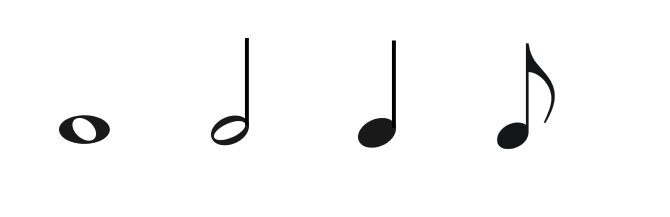
\includegraphics[height=10mm, width=25mm]{z_images/3_methodes/figures_de_notes.png}
\end{figure}
Une figure de note\cite{danhauser} de musique réunit plusieurs critères\footnote{\url{https://fr.wikipedia.org/wiki/Note_de_musique}} :
\begin{itemize}
	\item Une tête de note :\\
	Sa position sur la portée indique la hauteur de la note. La tête de note peut aussi indiquer la durée mais rarement en batterie en raison des symboles qui représentent les instruments.
	\item Une hampe :\\
	Indicatrice d’appartenance à une voix en fonction de sa direction et indicatrice d’une durée représentée par sa présence ou non (ronde ou blanche)
	\item Un crochet : La durée d’une note est divisée par deux à chaque crochet ajouté à la hampe d’une figure de note.
\end{itemize}
\begin{figure}[h]
	\centering
	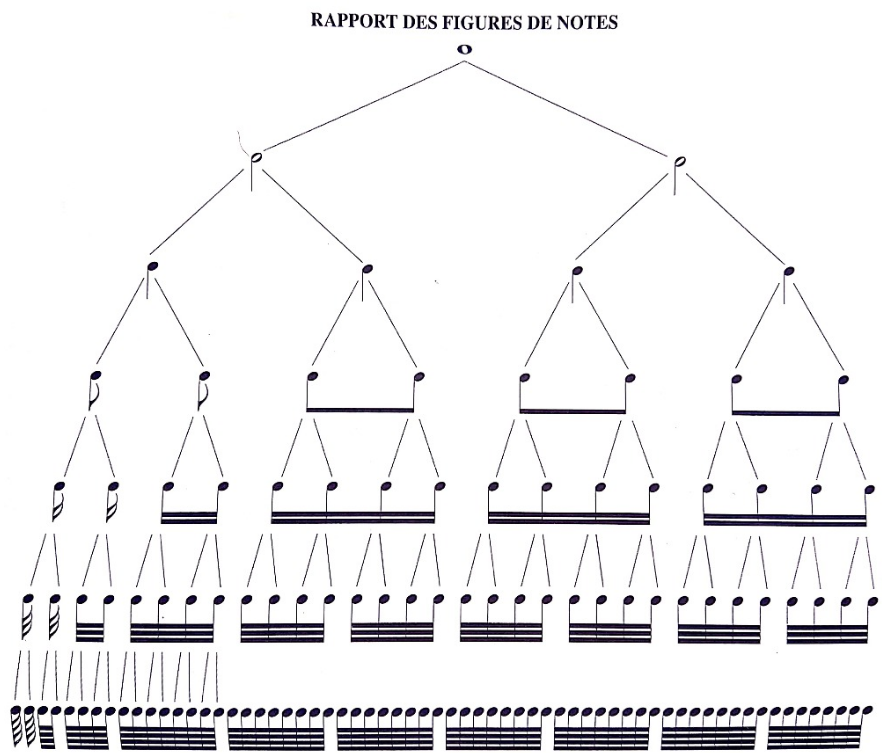
\includegraphics[height=50mm, width=80mm]{z_images/3_methodes/rapport_figures_notes.png}
	\caption{Rapport des figures de notes}\cite{danhauser}
\end{figure}
\subsection{Hauteurs et têtes de notes}
Pour la transcriptions, nous proposons une notation inspirée des méthodes agostini[ref] (et juskowiak[ref]), car nous trouvons la position des éléments cohérente et intuitive :\\
La caisse claire est centrale sur la portée et sur la batterie (au niveau de la ceinture, elle conditionne l’écart entre les pédales et aussi la position de tous les instruments basiques d’une batterie). 
Tous ce qui en dessous de la caisse-claire est en dessous de la ceinture (pédales, tom basse). Pareil pour au-dessus.\\
ainsi que l’organisation des éléments en hauteur (toms, cymbales, etc.).
On pensera en terme de symétrie la répartition des éléments par rapport au point central que constitue la caisse claire.\\
Cette symétrie s’opère en trois dimensions :
\begin{itemize}
	\item Les hauteurs en terme de fréquences ;
	\item La hauteur physique des éléments :\\
	Du bas vers le haut : pédales, toms et caisse, cymbales
	\item L’ergonomie, qui hiérarchise l’importance des éléments sur la portée (caisse claire au centre, hh-pied et ride sont aux deux extrémités).
\end{itemize}
\begin{figure}[!h]
	\centering
	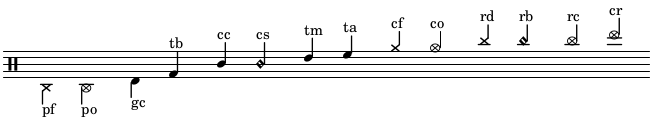
\includegraphics[height=25mm, width=130mm]{z_images/description_notation/notes.png}
	\caption{Hauteur et têtes de notes}
\end{figure}
\subsection{Nuances}
\begin{figure}[!h]
	\centering
	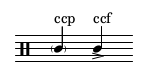
\includegraphics[height=20mm, width=35mm]{z_images/description_notation/nuances.png}
	\caption{Nuances}
\end{figure}
Bien expliquer les accents, remplacer p et f par g et a\\
$\Rightarrow$ nuance VS articulation\

\subsection{Durées}
Basé sur \cite{jacquemard:hal-01134096} et sur \cite{jacquemard:hal-01403982}\\
Pour la plupart des instruments mélodiques, la liaison et le point sont les deux seules possibilités en cas d’équivalence rythmique pour des notes dont la durée de l’une à l’autre est ininterrompue. Mais puisque les durées des notes n’ont pas d’importance en batterie, l’usage des silences pour combler la distance rythmique entre deux notes devient possible.\\
Ceci pris en compte, et étant donné que les indications de durée dans les têtes de notes ne sont pas pratique en batterie (les symboles « x » des cymbales ne
peuvent pas porter d’indication de durée dans la tête de notes\footnote{Certains logiciels le permettent mais leur lecture reste peu aisée}), l’écriture à l’aide de silences sera privilégiée comme indication de durée sauf dans les cas où cela reste impossible. Ce choix à pour but de n’avoir qu’une manière d’écrire toutes notes, que leurs têtes de notes soit modifiées ou non.\\\\
\textit{Exemple blanche vs noire + soupir}\\

Les cymbales-crash et les ouvertures de charley constituent les seusl cas qui excluent cette option. Le charley car ses ouvertures/fermetures sont presque toujours quantifiées et les cymbales-crash car elles peuvent être arrêtées à la main de manière quantifié aussi mais ce cas est très rare, nous allons donc nous concentrer sur les ouvertures de charley et considérer les crashs comme des événements sans durée.\\
Les fermetures du charley sont notées soit par un silence (correspondant à une fermeture de la pédale), soit par un écrasement de l’ouverture par un autre coup de charley fermé, au pied ou à la main.
\begin{figure}[!h]
	\centering
	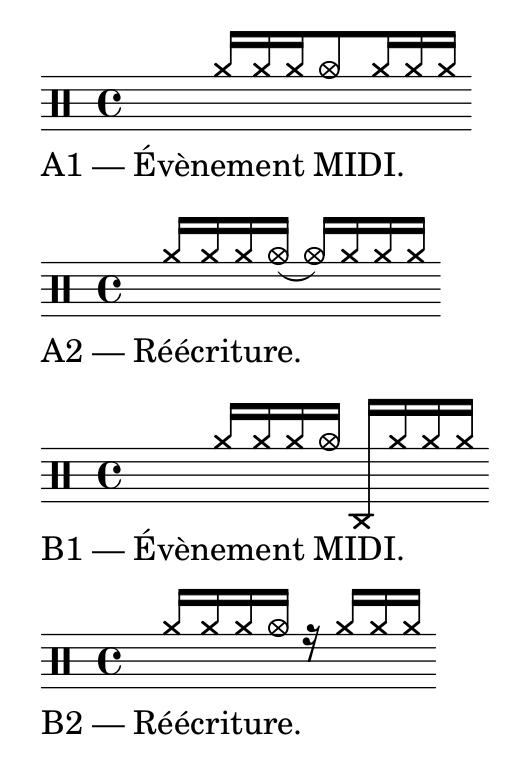
\includegraphics[height=80mm, width=60mm]{z_images/reecriture/exemples_charley_1.png}
	\caption{Durées}
	\label{duree_hh}
\end{figure}\newpage
\subsection{Voix}
Plusieurs écritures sont possibles pour un même rythme :\\\\
\begin{figure}[!h]
	\centering
	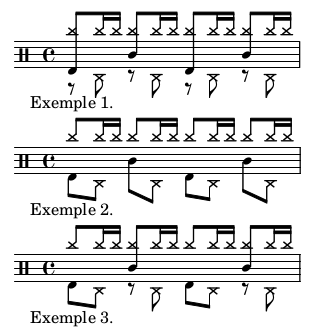
\includegraphics[height=65mm, width=60mm]{z_images/description_notation/separation/0_exemples_separation.png}
	\caption{Séparation des voix}
	\label{sep_voix}
\end{figure}\\
Sur la figure \ref{sep_voix}, il faudra faire un choix entre les exemples 1, 2 et 3 qui sont trois façon d’écrire la même chose. Ce choix se fera en fonction de la lisibilité, de quelles instruments auront des phrasés plus ou moins chargé et/ou variés, auquel cas on les mettra dans une seule voix afin de ne pas charger la partition, etc.
Ainsi l’arbre syntaxique de départ sera divisé en autant d’instruments qui le constituent et les voix seront regroupées de manière cohérentes.
\section{Modélisation pour la transcription}
\label{modelisation_transcription}
\subsection{Les pitchs}
\begin{table}[h]
	\centering
	\begin{tabular}{|c|c|c|} \hline
		Codes & Instruments & Pitchs \\ \hline
		cf & charley-main-fermé & 22, 42 \\
		co & charley-main-ouvert & 26 \\
		pf & charley-pied-fermé & 44 \\
		rd & ride & 51 \\
		rb & ride-cloche (bell) & 53 \\
		rc & ride-crash & 59 \\
		cr & crash & 55 \\
		cc & caisse-claire & 38, 40 \\
		cs & cross-stick & 37 \\
		ta & tom-alto & 48, 50 \\
		tm & tom-medium & 45, 47 \\
		tb & tom-basse & 43, 58 \\
		gc & grosse-caisse & 36 \\ \hline
	\end{tabular}
	\caption{Pitchs et instruments}
\end{table}
Pas de charley pied ouvert…
\subsection{La vélocité}
\begin{table}[h]
	\centering
	\begin{tabular}{|c|c|c|c|} \hline
		Codes & Instruments & Pitchs & Vélocité \\ \hline
		cop & charley-main-ouvert & 46 & ? \\ \hline
	\end{tabular}
	\caption{Vélocité et nuances}
\end{table}
Nous ne prendrons en compte la vélocité que pour la cc, les toms et les cymbales jouées aux mains. Les nuances de grosse caisse et charley aux pieds sont le plus souvent insignifiantes, elles ne sont marquées sur le figure qu’à titre indicatif.
Si la vélocité est en dessous de 40, il s’agit de ghost-notes : la tête de note devra être entouré de parenthèses et le suffixe \textit{p (piano)} devra être ajouté au codes de l’instrument. (Voir ccp ci-dessus.)
Si la vélocité est au dessus de 90, il s’agit de notes accentuées : le symbole « > » et le suffixe \textit{f (forte)} devra être ajouté au codes de l’instrument. (Voir ccf ci-dessus.)
Lorsque la vélocité va de 40 à 89, on considèrera le volume comme normal et aucun symbole supplémentaire ne sera ajouté à la note.\\\\

%\subsubsection{Les dilemmes}
Le charley de pitch 46 est considéré comme le charley ouvert joué à la main sur le haut de la cymbale mais souvent, ça correspond au geste « tranche-olive » de la baguette lorsque le batteur accentue avec la tranche et joue moins fort avec l’olive sur le plat de la cymbale. Je vais dans un premier temps considérer le pitch comme \textbf{charley-main-ouvert-piano} (ghost-note)
\subsection{Les arbres de rythmes}
Voici une représentation de la figure \ref{sep_voix} en arbre de rythme avec les codes de chaque instrument :\\\\
\Tree[ [ [rd\\gc ][ [rd\\pf ][rd ]]]
[ [rd\\cc ][ [rd\\pf ][rd ]]]
[ [rd\\gc ][ [rd\\pf ][rd ]]]
[ [rd\\cc ][ [rd\\pf ][rd ]]] ]\\\\\\
Ci-dessous, le même arbre dont les codes des instruments sont remplacés par leurs données midi respectives :\\\\
\Tree[ [ [51\\36 ][ [51\\44 ][51 ]]]
[ [51\\38 ][ [51\\44 ][51 ]]]
[ [51\\36 ][ [51\\44 ][51 ]]]
[ [51\\38 ][ [51\\44 ][51 ]]] ]\\\\\\
Cet arbre représente un rythme unique dont les possibilités de notation sur une partition sont théoriquement multiples. Les trois exemples de la figure 3.4 peuvent-être représentés par les arbres ci-dessus.
\section{Qparse}
\textit{Mettre ici un schéma de la chaîne de traitement de qparse (workflow)}\\
Pb du MIDI avec qparse entrée ON-OFF $\Rightarrow$ sortie 1 seul symbole.\\
Qparse produit une partition musicale en prenant en entrée une performance musicale symbolique (par exemple un fichier MIDI) et un automate à arbre pondéré décrivant un langage de rythmes préférés (grammaire pondérée). La quantification des rythmes est basée sur des algorithmes d’analyse syntaxique applicables sur des automates arborescents.\footnote{\url{https://qparse.gitlabpages.inria.fr}}
En entrée : midi (séquence d’événements datés (piano roll) accompagné d’une grammaire pondérée)\\
$\Rightarrow$ parsing\\
$\Rightarrow$ global parsing tree\\
$\Rightarrow$ RI (Représentation Intermédiaire) arbres locaux par intruments\\
$\Rightarrow$ Sortie (xml, mei, lilypond,… )\\
Minimiser la distance entre le midi et la représentation en arbre.\\
\textbf{Un des problèmes de Qparse était qu’il était limité au monophonique.}
$\Rightarrow$ \textit{Expliquer ici les limites du monophonique…}
%\subsection{Les Jams}
%Regroupement par nature des notes qui forment un accord.
\subsection{La grammaire pondérée}
La grammaire pondérée qui accompagne le MIDI en input est une grammaire hors-contexte pondérée. Chaque règle comporte un poid qui sert à favoriser certains rythmes plutôt que d’autres.\footnote{\url{https://qparse.gitlabpages.inria.fr/docs/scientific/}}
\subsection{Le parsing}
Le parsing du midi donné en input crée une représentation symbolique sous forme d’arbre de rythme.\\
Ici $\Rightarrow$ exemple avec :\\
3bars\_fill\_groove-016.mid $\Rightarrow$ arbre\\
\subsection{La réécriture}
\subsubsection{Séparation des voix}
\subsubsection{Simplification}
Ici, description basique des règles de réécriture 
\section{Les systèmes}
\label{systemes_methodes}
Un système est la combinaison d’un ou plusieurs éléments qui jouent un rythme en boucle (motif) et d’un autre élément qui joue un texte rythmique variable mais respectant les règles propre au système (gamme).\\

Système = motif + gamme/texte\\
motif = rythmes coordonnés joués avec 2 ou 3 membres en boucle (reparti sur 1 ou 2 voix)\\
gamme/texte = rythme irrégulier joué avec un seul membre sur le motif (Réparti sur 1 voix). La gamme d’un système considère l’ensemble des combinaisons que le batteur pourrait rencontrer en interprétant un texte rythmique à l’aide du système.\\

Nous partirons de propositions génériques de systèmes (environs trois systèmes dans différents styles de batterie) que nous tenterons de détecter dans le jeu de données groove.\\

Quatre systèmes standards :
\begin{itemize}
	\item binaire
	\item ternaire (shuffle, afro, rock)
	\item jazz
	\item afro-cubain\\
\end{itemize}

Nous travaillerons aussi sur la détection de répétitions sur plusieurs mesures afin de pouvoir corriger des erreurs sur une des mesures qui aurait dû être identique aux autres mais qui présente des différences.

\subsubsection{Intérêt des systèmes}
\textit{\textbf{Détection d’indication de mesure et choix de grammaire pondérée}}\\
Il faut prendre en compte l’existence potentielle de plusieurs grammaires \textit{(un fichier wta par grammaire)} chacunes dédiées à un type de contenu MIDI. Le choix d’une grammaire pondérée doit être fait avant le parsing puisque qparse prends en entrée un fichier MIDI et un fichier wta.\\
Pour les expériences effectuées avec le Groove MIDI Data Set, le style et l’indication de mesure sont récupérables par les noms de fichiers MIDI, mais il faudra par la suite les trouver automatiquement sans autres indications que les données MIDI elles-mêmes.\\
En conséquence, les motifs des systèmes devront être recherchés sur l’input \textit{(fichiers MIDI)} avant le lancement du parsing, afin de déterminer la métrique en amont en vu de sélectionner la grammaire pondérée \textit{(fichier wta)} adéquate pour le parsing. Nous pensons que cette tâche devrait être effectuée en Machine Learning.
\textbf{Les systèmes devront être matchés sur l’input MIDI}
\begin{itemize}
	\item Définir une métrique ;
	\item Réécriture : séparation des voix ;
	\item Réécriture : Set de règles spécifiques de simplification.
\end{itemize}

Il faudra créer un ensemble de systèmes comprenant leurs règles spécifiques de réécriture (séparation des voix et simplifications).
3 grandes catégories :
\begin{table}[h]
	\centering
	\begin{tabular}{|c|c|c|c|c|} \hline
		Systèmes & Métriques & Subdivisions & Possibles & nb voix \\ \hline
		binaires & simple & doubles-croches & triolets, sextolets & 2 \\
		jazz & simple & triolets & croches et doubles-croches & 2 \\
		ternaires & complexe & croches & duolets, quartelets & 2 \\
		afros-cubains & simple & croches & - & 3 \\ \hline
	\end{tabular}
	\caption{Sytèmes}
\end{table}

\begin{itemize}
	\item ternaire (mesures complexes, principalement croches, noire pointées, duolets et quartelets possibles)
	\item afro-cubain (mesure)
	\item Tout transcrire avec lilypond et en arbres d’analyse syntaxique.
	\item Créer les arbres de voix séparées.
	\item Écrire les règles de réécriture.
	\item Créer les arbres de voix séparées simplifiés (rewriting).\\	
\end{itemize}

Pour la \textbf{séparation des voix} et la \textbf{définition des métriques}, nous nous intéresserons principalement à la partie \textit{motif} des systèmes qui seront présentés. La partie \textit{texte} nous intéressera plus pour les \textbf{combinaisons de réécritures}.
\newpage
\subsubsection{Réécriture — Pour la séparation des voix}

\textbf{Motif 4-4 binaire}\\\\
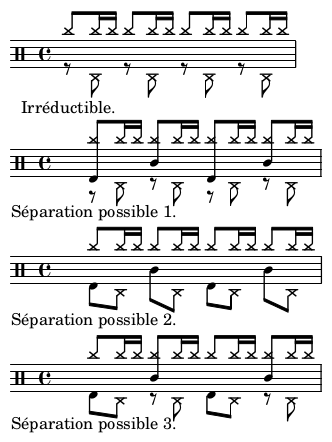
\includegraphics[height=60mm, width=40mm]{z_images/description_notation/separation/1_separation_4-4_binaire.png}\\\\
Ici, le système est construit sur un modèle rock en 4/4 : after-beat sur les 2 et 4 avec un choix de répartition des cymbales type fast-jazz. Le système est constitué par défaut du motif ride/ch-pf/cc et d’un texte joué à la grosse-caisse. La troisième séparation proposée est privilégiée car elle répartit selon 2 voix, une voix pour les mains (ride + cc) et une voix pour les pieds (ch-pf + gc). Ce choix paraît plus équilibré car deux instruments sont utilisés par voix et plus logique pour le lecteur puisque les mains sont en haut et les pieds en bas.\\
%D’autres choix d’écriture auraient été possibles :
%\begin{itemize}
%	\item Toutes les hampes en haut ;
%	\item Combinaison motif 1 et 2 en donnant 2 directions aux hampes de la cc).\\
%\end{itemize}

\textbf{Motif 4-4 jazz}\\\\
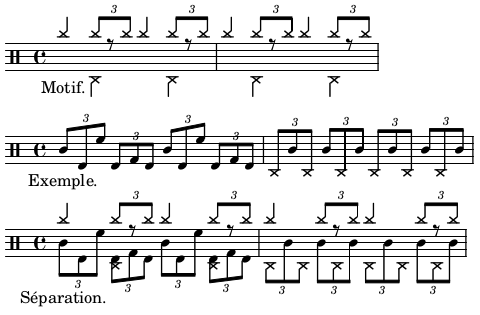
\includegraphics[height=45mm, width=60mm]{z_images/description_notation/separation/2_separation_4-4_jazz.png}\\\\
Dans la plupart des méthodes, le charley n’est pas écrit car considéré comme évident en jazz traditionnel. Ce qui facilite grandement l’écriture : la ride et les crash sur la voix du haut et le reste sur la voix du bas. Ici, le partie prit et de tout écrire. Dans l’exemple ci-dessus, les mesures 1 et 2 combinées avec le \textit{motif} de la première ligne, sont des cas typiques de la batterie jazz. Tout mettre sur la voix haute serait surchargé. De plus, la grosse caisse entre très souvent dans le flot des combinaisons de toms et de caisse claire et son écriture séparée serait inutilement compliquée et peu intuitive pour le lecteur. Le choix de séparation sera donc de laisser les cymbales en haut et toms, caisse-claire, grosse-caisse et pédale de charley en bas.\\

\textbf{Système 4-4 afro-cubain}\\\\
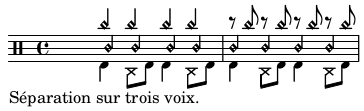
\includegraphics[height=25mm, width=80mm]{z_images/description_notation/separation/3_separation_afro-cubain.png}\\

\subsubsection{Pour la reconnaissance de la métrique}
\textit{\textbf{12/8 vs 4/4 ternaire}}\\\\
\textbf{Motif 12/8}\\\\
%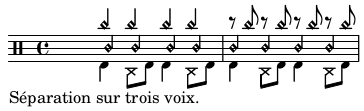
\includegraphics[height=30mm, width=100mm]{z_images/1_description_notation/separation/separation_2.png}\\\\

\subsubsection{Pour les règles de réécriture}
Les textes qui accompagnent les motifs étayent toutes les combinaisons d’un systèmes.\\


%\subsubsection{Construction des systèmes pour les expérimentations}
%\subsubsection{La réécriture des évènements MIDI pour la batterie}



\textbf{Exemples à écrire en arbre :}\\
\begin{itemize}
	\item 
	SI (pas pf) ET (note sur un temps suivie de note en l’air) :\\
	$\Rightarrow$ (Temps1 : Note pertinente) + (Temps2 : Silence pertinent + Note pertinente.)\\
	\item
	Si (po ou co) déborde sur le temps suivant :\\
	$\Rightarrow$ Liaison car marchera dans tous les cas même la où le point ne marchera pas (voir A2).\\
	\item
	Une blanche sera écrite noir + soupir.\\\\
\end{itemize}

%\newpage
%\subsubsection{Expérience 2}
%\textbf{Partition de référence pour l’ouput}
%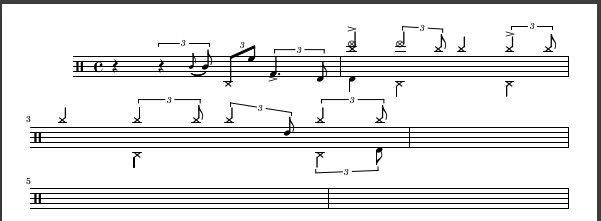
\includegraphics[height=50mm, width=160mm]{z_images/4_experimentations/experience_2/partition.png}\\\\
%\textit{En cours…}
\section*{Conclusion}
Bilan sur les différentes méthodes employées et la contribution que cela représente.